From the results in the previous section, it can be seen that the performance of the Classifier module over the test set was better than the performance of the baseline.
It shows that considering such features that rely on computation of relevance of the content within a sentence can give much better results than considering just the textual content of the sentence.
This can be attributed to the fact that in the Classification module, the features extracted for classification of the sentence captured the relevance of the the words (that appear in that sentence) with respect to the entire document.

Although the test set consisted of sentences that were all selected from the top of the output of the TextRank algorithm, the negative sentences in the training set were picked from the bottom of the output of the TextRank algorithm.
From the confusion matrix in Table 4.2 we can see that the negative predictive value (which indicates how well negative samples are classified) of the trained model is 62.2\% and the specificity (which indicates the fraction of true negative samples that were identified correctly) is 93.1\%.
This shows that the trained model is able to identify the negative sentences in most of the cases.
This helps in validating the decision to pick negative samples as the the lowest ranked sentences in the document for training.

Despite the accuracy of the trained model in predicting negative sentences, it is still more important to judge the classifier based on its efficiency to classify positive sentences correctly.
This is because the aim of the task is to highlight sentences that could be important, which are positive sentences in the data set.
A close analysis of the sentences in the test set, their respective feature values and the real and predicted classes for each helped in understanding the shortcomings of the model.
Since the importance metric sec-tf-idf is calculated by considering the section (as annotated in the document structure) as a document and the whole document as the corpus, the value of the same word differs with its occurance in different sections.

Figure 7.1 shows the dependency parse of a positive sentence which was classified correctly by the trained model.
The values of the three features have also been mentioned beside the words that represent the subject, the verb and the object phrases.
Although it is an estimate in accordance with the plots shown in Figure 4.1, it can be seen that these values are high enough to be considered as positive samples.

\begin{figure}[h]
\centering
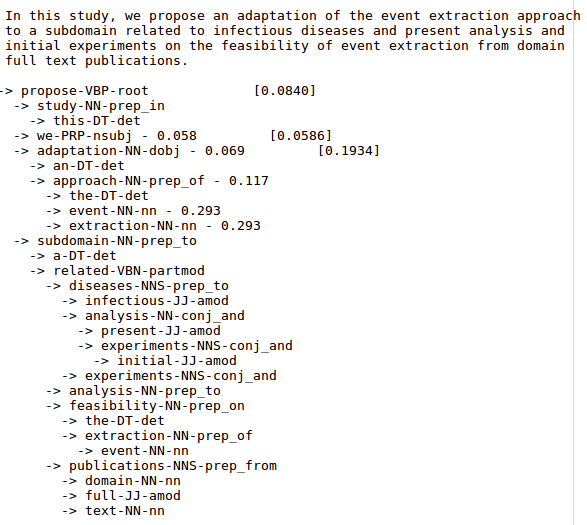
\includegraphics[width=0.7\linewidth, height=7cm]{discuss1} 
\caption{Dependency Parse for a positive sentence with sec-tf-idf values}
\label{fig:dep-discus1}
\end{figure}

\begin{figure}[h]
\centering
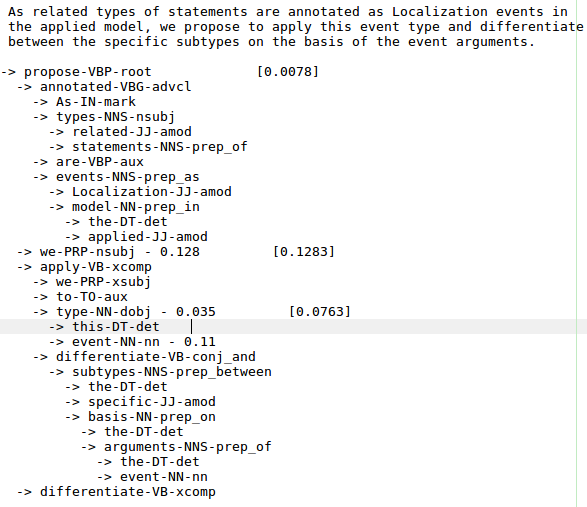
\includegraphics[width=0.7\linewidth, height=7cm]{discuss2} 
\caption{Dependency Parse for a negative sentence with sec-tf-idf values}
\label{fig:dep-discus2}
\end{figure}

Figure 7.2 shows the dependency parse of another positive sample which was classified incorrectly by the trained model as a negative sentence.
Here it can be seen that the value of the word 'propose' is 0.007 which is quite low where as the value of the same word in Figure 7.1 is 0.08.
The values of this word are different because the two sentences appear in different sections.

I used the value of the word 'propose' from the first sentence as a feature for the second sentence since in both the sentences this word is the main verb and is used for that feature.
With this and the other two values of subject and object phrases from the second sentence, I created a feature vector and used the trained model to classify it.
The feature vector was classified as a positive sample.

From the above discussion it can be seen that although the feature sec-tf-idf can be used to perform classification that could lead to imporvement over the baseline, it can still miss out on positive sentences.
Although the precision of the train model using this novel metric is sufficiently good, the recall is poor.
For summarization, it is important to find sentences that could be included in the summary.
Hence, there is a need to improve the features to help better map the importance of words in a sentence.

A further improvement that has been proposed for future work is to add a linear component to the features being calculated.
a feature that measure a more general significance of words can be used.
This can be measure over large corpus which need not necessaily be a collection of scientific articles.
A possible suggestion is the use of Google n-gram data set.
The feature could be a linear combination of the sec-tf-idf value as well as Google n-gram data set.